\documentclass[twoside,twocolumn]{article}
\usepackage{amsmath}
\usepackage{blindtext} % Package to generate dummy text throughout this template 
\usepackage{graphicx}
\usepackage{natbib}

\usepackage[sc]{mathpazo} % Use the Palatino font
\usepackage[T1]{fontenc} % Use 8-bit encoding that has 256 glyphs
\linespread{1.05} % Line spacing - Palatino needs more space between lines
\usepackage{microtype} % Slightly tweak font spacing for aesthetics

\usepackage[english]{babel} % Language hyphenation and typographical rules

\usepackage[hmarginratio=1:1,top=32mm,columnsep=20pt]{geometry} % Document margins
\usepackage[hang, small,labelfont=bf,up,textfont=it,up]{caption} % Custom captions under/above floats in tables or figures
\usepackage{booktabs} % Horizontal rules in tables

\usepackage{lettrine} % The lettrine is the first enlarged letter at the beginning of the text

\usepackage{enumitem} % Customized lists
\setlist[itemize]{noitemsep} % Make itemize lists more compact

\usepackage{abstract} % Allows abstract customization
\renewcommand{\abstractnamefont}{\normalfont\bfseries} % Set the "Abstract" text to bold
\renewcommand{\abstracttextfont}{\normalfont\small\itshape} % Set the abstract itself to small italic text

\usepackage{titlesec} % Allows customization of titles
\renewcommand\thesection{\Roman{section}} % Roman numerals for the sections
\renewcommand\thesubsection{\roman{subsection}}
\titleformat{\section}[block]{\large\scshape\centering}{\thesection.}{1em}{} % Change the look of the section titles
\titleformat{\subsection}[block]{\large}{\thesubsection.}{1em}{} % Change the look of the section titles

\usepackage{fancyhdr} % Headers and footers
\pagestyle{fancy} % All pages have headers and footers
\fancyhead{} % Blank out the default header
\fancyfoot{} % Blank out the default footer
\fancyhead[C]{FYS4150 $\bullet$ Project 2 $\bullet$ October 2016} % Custom header text
\fancyfoot[RO,LE]{\thepage} % Custom footer text

\usepackage{titling} % Customizing the title section

\usepackage{hyperref} % For hyperlinks in the PDF

%----------------------------------------------------------
%  COMMANDS
%---------------------------------------------------------

\newcommand{\nl}{
	
	\medskip
	\noindent
}
%--------------------------------------------

\newcommand{\SE}{Schroedinger equation }
\newcommand{\CI}{Coulomb interactions}
%----------------------------------------------------------------------------------------
%	TITLE SECTION
%----------------------------------------------------------------------------------------

\setlength{\droptitle}{-4\baselineskip} % Move the title up

\pretitle{\begin{center}\Huge\bfseries} % Article title formatting
	\posttitle{\end{center}} % Article title closing formatting
\title{FYS4150 - Project 2} % Article title
\author{%
	\textsc{Vegard R\o{}nning \& Heine H. Ness \& Sindre R. Bilden} \\[1ex] % Your name
	\normalsize University of Oslo \\ % Your institution
	\normalsize \href{mailto:vegard.ronning@fys.uio.no}{vegard.ronning@fys.uio.no}\ ; \href{mailto:h.h.ness@fys.uio.no}{h.h.ness@fys.uio.no}\ ; \href{mailto:s.r.bilden@fys.uio.no}{s.r.bilden@fys.uio.no}\\% Your email address
	\footnotesize \href{https://github.com/sindrerb/FYS4150-Collaboration/tree/master/Doc/Project2}{github.com/sindrerb/FYS4150-Collaboration/tree/master/Doc/Project2}
	%\and % Uncomment if 2 authors are required, duplicate these 4 lines if more
	%\textsc{Jane Smith}\thanks{Corresponding author} \\[1ex] % Second author's name
	%\normalsize University of Utah \\ % Second author's institution
	%\normalsize \href{mailto:jane@smith.com}{jane@smith.com} % Second author's email address
}
%----------------------------------------------------------------------------
\date{\today} % Leave empty to omit a date
\renewcommand{\maketitlehookd}{%
	\begin{abstract}
\vspace{-0.4cm} As tracers in medicine or qubits in quantum computing, utilizing quantum dots are hot topics in science. One advantage of quantum dots are their discrete energy levels which may be tuned by existing technology and knowledge. As a one particle problem, the quantum dot may be solved analytically as a particle in a three dimensional harmonic oscillator potential (HO), but the solution is almost impossible to find once multiple particles are confined in one single quantum dot. The project uses numerical methods to solve the eigenvalue problem of two electrons in a quantum dot and examines the impact of \CI on the system. The results shows that the impact of the \CI increases with a widening potential. 
\vspace{-0.5cm}
	\end{abstract}
}

%----------------------------------------------------------------------------

\begin{document}
	
	% Print the title
	\maketitle
	
	%----------------------------------------------------------------------------
	%	ARTICLE CONTENTS
	%----------------------------------------------------------------------------
\vspace{-2cm}
	\section{Introduction}\vspace{-0.4cm}
	\lettrine[nindent=0em,lines=2]{Q}uantum dots are promising field of science, with a wide range of applications. As a single particle system, the quantum dot is possible solve analytically by approximating it to a three dimensional HO-potential. Once the system consist of to two or more particles, it becomes very complex and is often not possible to solve analytically like the single particle system. It is possible to achieve a close approximate of a two particle system numerically by using Jacobi's method, that may be used to confirm experimental results or as an experiment by itself. This project consists of two main parts where the first is writing a program that utilizes Jacobi's method (presented in section \ref{sec:methods}, Methods) to solve the \SE (SE) numerically for a one particle in a three dimensional HO-potential as described in section \ref{sec:implementation}, Implementation. The numerical results will be compared to analytical results before proceeding to the second part which is to introduce a second particle and solve the system with and without \CI. The impact of the \CI is then calculated by studying the energy difference between the interacting and the non interacting case, where the results are presented and discussed in section \ref{sec:results}.
	%----------------------------------------------------------------------------
	\section{Methods}
	\label{sec:methods}
	\subsection{Jacobi's method}
	Jacobi's method is an iterative method which uses Jacobi's rotation matrix $\hat{S}$ a number of times to turn a symmetric, hermittian matrix $\hat{A}$ to a diagonal matrix $\hat{D}$.
	
	\begin{equation*}
	\hat{S}^T\hat{A}\hat{S} = \hat{S}^T_n\hat{S}^T_{n-1}\cdots\hat{S}^T_1\hat{A}\hat{S}_1\cdots\hat{S}_{n-1}\hat{S}_n = \hat{D}
	\end{equation*}
	
	\noindent
	The rotation matrix $\hat{S}_i$, where $i = 1,2\cdots n$, has the form of an identity matrix with $c = \cos(\theta)$ and $s = \sin(\theta)$ in a symmetric fashion inside depending on which two elements in $\hat{A}$ is to be rotated. $n$ depends on the number of rotations needed to transform $\hat{A}$ to $\hat{D}$.   
	
	\begin{equation*}
	\hat{S} = \begin{bmatrix}
	1 & 0 & & \cdots & & & 0 \\
	0 & \ddots &  &  & & & \\
	&  & c & \cdots & s & &\\
	\vdots & & \vdots & \ddots & \vdots & &\vdots\\
	& & -s & \cdots & c & &\\
	& & & & &\ddots & 0\\
	0 & & & \cdots & & 0 & 1
	\end{bmatrix}
	\end{equation*}
	
	\noindent
	In this assignment we will use Jacobi's method to solve a eigenvalue problem. The eigenvalues ($\lambda$) are preserved using the this method but the eigenvectors are generally not, only the orthogonality of the eigenvectors are preserves. The eigenvalue problem $\hat{A}\vec{x} = \lambda\vec{x}$ then becomes 
	
	\begin{align*}
	(\hat{S}^T\hat{A}\hat{S})(\hat{S}^T\vec{x}) &= (\hat{S}^T\lambda\hat{S})(\hat{S}^T\vec{x})\\
	\hat{D}(\hat{S}^T\vec{x}) &= \lambda(\hat{S}^T\vec{x})
	\end{align*}
	
	
	\nl
	If $\hat{A}$ is composed of elements $a_{ij}$ and matrix $\hat{B}$ of elements $b_{ij}$. 
	One rotation $\hat{S}_i^T\hat{A}\hat{S}_i = \hat{B}$ can be done with an algorithm. 
	\nl
	First the largest non-diagonal element $a_{kl}$ has to be located then the element will be set to zero. Since the matrix is symmetric and $\hat{S}$ is designed as it is, the element $a_{lk}$ will be subject to the same operation as $a_{kl}$.
	
	\begin{equation*}
	b_{kl} = b_{lk} = (a_{kk}-a_{ll})cs + a_{kl}(c^2-s^2) = 0
	\end{equation*}
	
	The equation
	
	\begin{equation*}
	(a_{kk}-a_{ll})cs + a_{kl}(c^2-s^2) = 0
	\end{equation*}
	
	
	\noindent
	Is solved by using $\Gamma = \frac{a_{ll} - a_{kk}}{2a_{kl}}$ and $t = \frac{s}{c}= \tan(\theta)$ to get the second order polynomial
	
	\begin{equation*}
		t^2 + 2\Gamma t-1 = 0
	\end{equation*}
	
	This gives a solutions for the trigonometrical expression.
	
	\begin{align*}
	&t = -\Gamma\pm \sqrt{1+\Gamma^2}\\
	&c = \frac{1}{\sqrt{1 + \Gamma^2}}\\
	&s = tc
	\end{align*}
	
	To avoid problems where $\Gamma$ gets large and possible loss of numerical precision we rewrite $t = \frac{1}{\Gamma + \sqrt{1+\Gamma^2}}$.
	\nl
	Rotation algorithm is solved with the previously given solutions for $t$,$c$ and $s$ by a simple algorithm. 
	
	\begin{align*}
	&b_{ii} = a_{ii} &|i\neq k,l\\
	&b_{ik} = a_{ik}c - a_{il}s &|i\neq k,l\\
	&b_{il} = a_{il}c + a_{ik}s &|i\neq k,l\\
	&b_{kk} = a_{kk}c^2 - 2a_{kl}cs + a_{ll}s^2&\\
	&b_{ll} = a_{ll}c^2 + 2a_{kl}cs + a_{kl}s^2&\\
	&b_{kl} = b_{lk} = 0&
	\end{align*}
	
	\noindent
	
	Here $i = 1,2\cdots n$ is the iteration variable and $k$ and $l$ are parameter belonging to the element in rotation.
	
	\subsection{Abel-Ruffini Impossibility Theorem}
	
	The eigenvalue problem $\det(\hat{A}-\lambda \hat{I})\vec{x} = 0$ of a matrix $\hat{A}\in \mathbb{C}^{n\times n}$ is basically a problem of finding the roots of a polynomial $P(\lambda)$. 
	
	\begin{equation*}
	P(\lambda) = \prod_{i=1}^n(\lambda_i - \lambda)
	\end{equation*}
	
	\noindent
	The Abel-Ruffinis impossibility theorem states that not all polynomials of degree $n\geq 5$ can not be solved using roots alone and the solutions for these cases can only be approximated. \citep{compfys}
	\nl
	This implies that matrices $\hat{A}$ of large dimensions has to be solved numerically and is only possible to get an approximation for the eigenvalues with a chosen degree of numerical accuracy within the boundaries of the computer.
	
	\subsection{Unit tests}
	A unit test is a small block of code that tests parts of a program for calculation errors. This to ensure that the program runs as expected and delivers correct results throughout the program.
The unit tests used in this assignment are as follows.
	
	\subsubsection{Orthogonality test}
	
	The Jacobi method preforms orthogonal or unitary transformations to the matrix it operates on. That means the orthogonality of each column in a matrix $\hat{A}$ is conserved.\nl
	
	If $\hat{A}$ is a orthogonal matrix with orthogonal column vectors $\hat{A} = [\vec{a_1} \vec{a_2} \cdots \vec{a_n}  ]$ the dot product of any column vector can be described by a Kronecker delta $\delta_{ij}$.
	
	\begin{align*}
	\vec{a_i}^T \vec{a_j} = |a_i|^2\delta_{ij} =
	\begin{cases}
	|a_i|^2|i=j\\
	0\hspace{0.5cm}|i\neq j
	\end{cases}
	\end{align*}
	
	For a transformation done by a matrix $\hat{S}$ to be unitary, all vectors $\vec{w_i}$ produced by the transformation $\hat{S}\vec{v_i} = \vec{w_i}$ must also be orthogonal.
	
	\begin{align*}
	&\vec{w_i^T}\vec{w_j} = (\hat{S}\vec{v_i})^T\hat{S}\vec{v_j} = \hat{S}^T\vec{v_i}^T\hat{S}\vec{v_j} = \\ &\vec{v_i}^T\hat{S}^T\hat{S}\vec{v_j} = \vec{v_i}\vec{v_j} = \delta_{ij}
	\end{align*}
	
	\subsubsection{Normality test}	
	Since Jacobi's method preform unitary transformations to the matrix it operates on, the normality is conserved if the columns of $\hat{A}$ is normalized.\nl
	In this case Jacobi rotation is done on the identity matrix which is normalized by definition. Introducing the criteria $$col_i(\hat{A})^T\cdot col_i(\hat{A})=1$$ gives a brief indication of the conservation of normality which is important for the interpretation of the wavefunction.
	%----------------------------------------------------------------------------
	\section{Implementation}
	\label{sec:implementation}
	A quantum dot may be approximated to a three dimensional HO-potential. By assuming spherical symmetry, the radial part of the SE may be rewritten to
	\begin{align*}
	&-\dfrac{\hbar^2}{2 m} \left ( \dfrac{1}{r^2} \dfrac{d}{dr} r^2 \frac{d}{dr} - \dfrac{l (l + 1)}{r^2} \right )R(r)\\ 
	&\hspace{1cm}+ V(r) R(r)= E R(r).
	\end{align*}
	Where the potential $V(r)$ is known by the HO-potential $\frac{1}{2}kr^2$, with $k=m\omega^2$ and the quantum number $l$ describe the orbital momentum of the electron.
	The energies and oscillator frequency is given by
	\begin{align*}
	E_{nl} = \hbar\omega\left(2n+l+ \dfrac{3}{2} \right)
	\end{align*}
	where $n\in \mathbb N$, $l\in \mathbb N$ and $r \in [0,\infty)$. By rewriting $R(r)$ as $rR(r) = u(r)$ we get
	\begin{align*}
	&-\dfrac{\hbar^2}{2 m} \frac{d^2}{dr^2} u(r) + \left ( V(r) + \dfrac{l (l + 1)}{r^2}\dfrac{\hbar^2}{2 m} \right ) u(r)\\  
	&\hspace{6cm}=  E u(r)
	\end{align*}
	The expression can be further simplified by introducing the dimensionless variable $\rho = \frac{1}{\alpha}r$, setting $V(\rho) = \frac{1}{2}k\alpha^2\rho^2$, multiply with $\frac{2m\alpha^2}{\hbar^2}$ and set $l=0$ so that
	\begin{align*}
	-\frac{d^2}{d\rho^2} u(\rho) +\underbrace{ \frac{mk}{\hbar^2} \alpha^4}_{I}\rho^2u(\rho)  = \underbrace{\frac{2m\alpha^2}{\hbar^2}E}_{II}u(\rho)
	\end{align*}
	and finally setting I $=1$ and defining II $=\lambda$ the final form of the SE for one electron in a HO-potential can be written as
	\begin{align}
	-\frac{d^2}{d\rho^2} u(\rho) + \rho^2u(\rho)  = \lambda u(\rho)\label{eq:dimless}
	\end{align}
	Equation \ref{eq:dimless} may be discretized and solved numerically as a matrix eigenvalue problem were $V_i=\rho_i^2$. 
	\begin{equation}
	-\frac{u_{i+1}-2u_i+u_{i-1}}{h^2}+V_iu_i = \lambda u_i \label{eq:disk1}
	\end{equation}
	\subsubsection{Two particle system}
	By introducing another electron, the system consists two particles in the potential and the interactions between them.
	SE for two electrons with no Coulomb interactions can be written as
	\begin{align*}
	&\left(  -\frac{\hbar^2}{2 m}\nabla^2+ \frac{1}{2}k(r_1^2+r_2^2)\right)u(r_1,r_2)= E u(r_1,r_2)\end{align*}
	This can be rewritten by introducing the relative coordinate $\textbf{r} = \textbf{r}_1-\textbf{r}_2$ and the center-of-mass(COM) coordinate $\textbf{R} = \frac{1}{2}(\textbf{r}_1 + \textbf{r}_2)$. The radial SE is then
	\begin{align*}
	&\left(  -\frac{\hbar^2}{m} \frac{d^2}{dr^2} -\frac{\hbar^2}{4 m} \frac{d^2}{dR^2}+ \frac{1}{4} k r^2+  kR^2\right)u(r,R)\\  &\hspace{5.5cm}= E u(r,R)
	\end{align*}
	The ansatz for the wavefunction $u(r,R) = \psi(r)\phi(R)$ makes it possible to separate the equation for \textbf{r} and \textbf{R} so that the energy is the sum of the relative energy and the COM-energy($E=E_r+E_R$).
	Taking the repulsive Coulomb interaction 
	\begin{align*}
	V_(r_1,r_2) = \dfrac{\beta e^2}{|\textbf{r}_1-\textbf{r}_2|} = \dfrac{\beta e^2}{r}, \hspace{0.5cm} \beta e^2 = 1.44\ \text{eVnm}
	\end{align*}
	in to account the r-dependent part of the SE can be written as
	\begin{align*}
	\left(  -\frac{\hbar^2}{m} \frac{d^2}{dr^2}+ \frac{1}{4}k r^2+\frac{\beta e^2}{r}\right)\psi(r)  = E_r \psi(r)
	\end{align*}
	By now introducing the dimensionless variable $\rho = \frac{r}{\alpha}$ and repeating the same steps as for the one electron case we get
	\begin{align*}
	\hspace{-1.5cm}-\dfrac{d^2}{d\rho^2} \psi(\rho) + \dfrac{1}{4}\frac{mk}{\hbar^2} \alpha^4\rho^2\psi(\rho)+\underbrace{\dfrac{m\alpha \beta e^2}{\hbar^2}}_{I}\dfrac{1}{\rho}\psi(\rho)  = \underbrace{ \dfrac{m\alpha^2}{\hbar^2}E_r}_{II}\psi(\rho)
	\end{align*}
	To further simplify the equation we introduce the new frequency
	\begin{align*}
	\omega_r^2 = \dfrac{1}{4}\dfrac{mk\alpha^4}{\hbar^2}
	\end{align*}
	Setting I $= 1$ and II $=\lambda$ we arrive at the final form of SE for the two electron case
	\begin{align}
	-\dfrac{d^2}{d\rho^2} \psi(\rho) + \omega_r^2\rho^2\psi(\rho) +\dfrac{1}{\rho}\psi(\rho) = \lambda \psi(\rho)\label{eq:dimless2pt}
	\end{align}
	Like equation \ref{eq:dimless}, equation \ref{eq:dimless2pt} may be discretized into
	\begin{equation}
	-\frac{u_{i+1}-2u_i+u_{i-1}}{h^2}+V_iu_i = \lambda u_i\label{eq:disk2}
	\end{equation}
	Were the new potential $V_i=\omega_r^2\rho_i^2+\frac{1}{\rho}$. Both equation \ref{eq:disk1} and \ref{eq:disk2} may be rewritten to $\hat{H}\hat{u}=\lambda\hat{u}$ were $\hat{H}$ is a tridiagonal matrix with center diagonal $d_{ii}=\frac{2}{h^2}+V_i$ and the upper diagonal equal to the lower diagonal equal to $e_{ij}=\frac{-1}{h^2}$. These matrix eigenvalue problems may be solved by Jacobi's method.\nl
	
	Tests of conserved orthogonality and normality was done on a one electron system to ensure that the algorithm was correct, sample-matrices was written to a file and later tested for conserved orthogonality and normality in a Python script 
(\href{https://github.com/sindrerb/FYS4150-Collaboration/blob/master/Doc/Project2/unitTest.py}{unitTest.py}). Later a convergence test of the number of iterations was done to weight the accuracy and computational time. The algorithm was set to solve SE for a two particle system with $\omega_r$ equal to $0.01,0.5,1$ and $5$. Both with and without \CI{}.
All code and results are found in the GitHub repository \\
{\small \centering \href{https://github.com/sindrerb/FYS4150-Collaboration/tree/master/Doc/Project2}{github.com/sindrerb/FYS4150-Collaboration/}}
	\section{Results and discussion}
	\label{sec:results}
	Jacobi's method may require many iterations in order to reach a satisfying accuracy of the energies. Table \ref{tbl:convergence} from the convergence test of mesh points indicates that $N=500$ is a minimum requirement for a four digit accuracy but results also in a high computational time. Figure \ref{fig:iterations} shows the number of iterations for a given set of mesh points, assumed to be proportional to computation time.
	A number of mesh points $N=400$ results in a accuracy to approximately the third digit, which is thought to be accurate enough for the purpose of this experiment while  reducing the computational time drastically.\nl
	
	\begin{table}[h]
			\caption{Table showing the three lowest computed eigenvalues $\lambda$ with $N$ mesh points, compared to the exact $\lambda_0=3$,$\lambda_1=7$ and $\lambda_2=11$.}\label{tbl:convergence}
		\centering
		\begin{tabular}{|l|l|l|l|}\hline
			$N$ & $\lambda_0$ & $\lambda_1$ & $\lambda_2$\\ \hline
			10 & 2.68672 & 6.11302 & 11.0574\\
			50 & 2.98745 & 6.93692 & 10.8453\\
			100& 2.99687 & 6.98432 & 10.9617\\
			200& 2.99916 & 6.99610 & 10.9904\\
			300& 2.99961 & 6.99828 & 10.9958\\
			400& 2.99986 & 6.99903 & 10.9976\\
			500& 2.99993 & 6.99937 & 10.9986\\\hline
		\end{tabular}
	\end{table}
	\begin{figure}[p]
		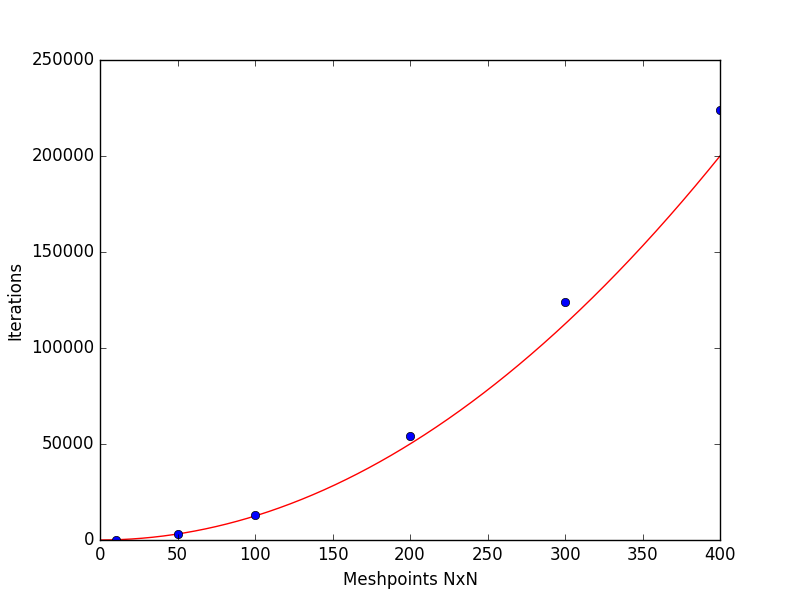
\includegraphics[width=0.5\textwidth]{figures/iterations.png} 
		\caption{Graph over the number of iterations for a given set of mesh points $N$. The solid red line is proportional to $N^2$ as a comparison.}\label{fig:iterations}
	\end{figure}
	\begin{figure}[p]
		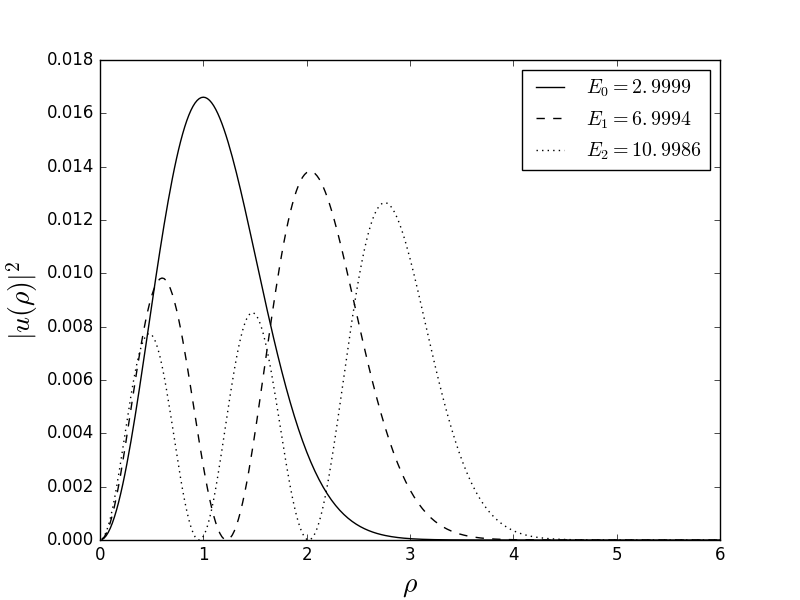
\includegraphics[width=0.5\textwidth]{../report/figures/eigenvecs123.png} 
		\caption{The first three eigenstates with their respective eigenstates in a harmonic oscillator with one particle, computed with $N=500$ mesh points.}\label{fig:eigenstates}
	\end{figure}
	\begin{table}[p]
			\caption{Table showing the energy of the ground state in a two particle system with and without \CI. The impact is defined by the energy difference of the systems divided by the energy of the interacting system. The energies are rounded to the third digit.}\label{tbl:Coulomb}
		\begin{tabular}{|l|l|l|l|}\hline
			$\omega_r$ & Interaction & No Interaction & Impact\\ \hline
			0.01 & 0.105 & 0.030 & 0.72\\
			0.25 & 1.250  & 0.750 & 0.40\\
			0.50 & 2.230 & 1.500 &  0.33\\
			1.00 & 4.058 & 3.000 &  0.26\\
			2.50 & 9.211 & 7.500 & 0.19\\
			5.00 & 17.448 & 15.000 & 0.14\\ \hline
		\end{tabular}
	\end{table}
	Results from the computation of the two particle systems is given in Figure \ref{fig:fq001} $-$ \ref{fig:fq500}, where it is a clear correspondence between the $\omega_r$ and the \CI. A high $\omega_f$ results in a narrow potential and a confinement of the electrons, in this narrow potential the \CI was thought to give a great impact on the wavefunction but Figure \ref{fig:fq500} contradicts this hypothesis. Figure \ref{fig:fq001} does also show an unexpected behavior where the \CI has a greater impact in the electrons than expected. A relation between the energies of the systems with and without \CI is given in Table \ref{tbl:Coulomb}. The behavior may be explained by the fact that $V_{Coulomb}=\frac{\beta}{r}$ diverge while $r$ goes to zero. In a narrow potential, the \CI are large but does not overpower the confinement of the potential. While widening the potential, the confinement decreases more rapidly than the \CI.
	\begin{figure}[p]
		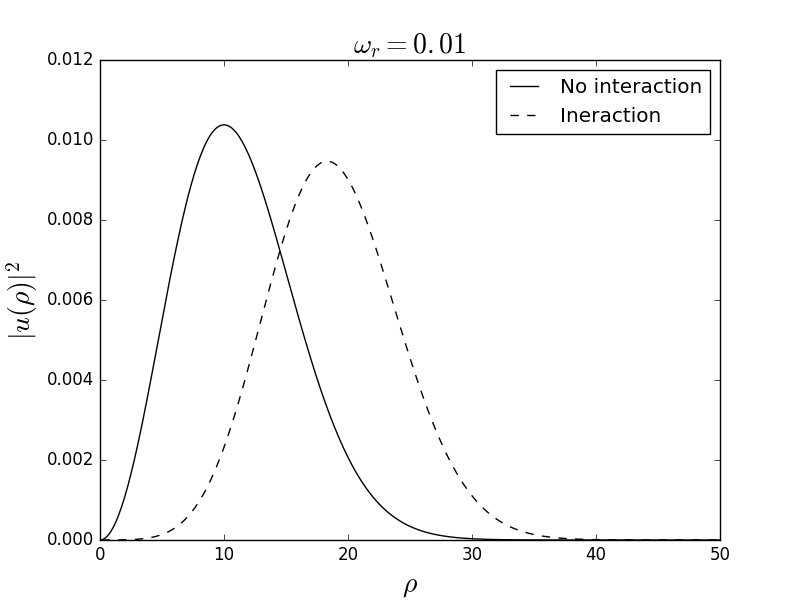
\includegraphics[width=0.45\textwidth]{../report/figures/freq001.png} 
		\caption{Comparison of the wavefunction with and without Coulomb interactions in a HO-potential where $\omega_r=0.01$}\label{fig:fq001}
	\end{figure}
	
	\begin{figure}[p]
		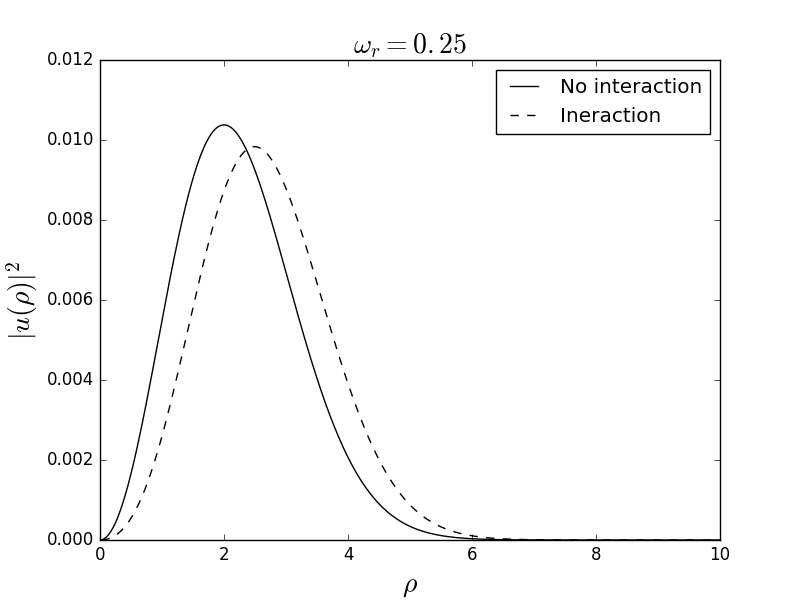
\includegraphics[width=0.45\textwidth]{../report/figures/freq025.png} 
		\caption{Comparison of the wavefunction with and without Coulomb interactions in a HO-potential where $\omega_r=0.25$}\label{fig:fq025}
	\end{figure}
	\begin{figure}[p]
		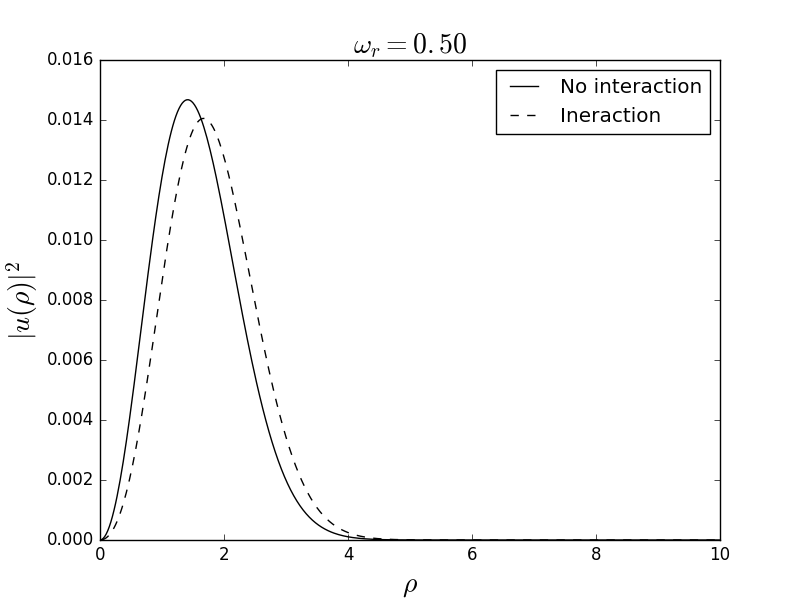
\includegraphics[width=0.45\textwidth]{../report/figures/freq050.png} 
		\caption{Comparison of the wavefunction with and without Coulomb interactions in a HO-potential where $\omega_r=0.5$}\label{fig:fq050}
	\end{figure}
	
	\begin{figure}[p]
		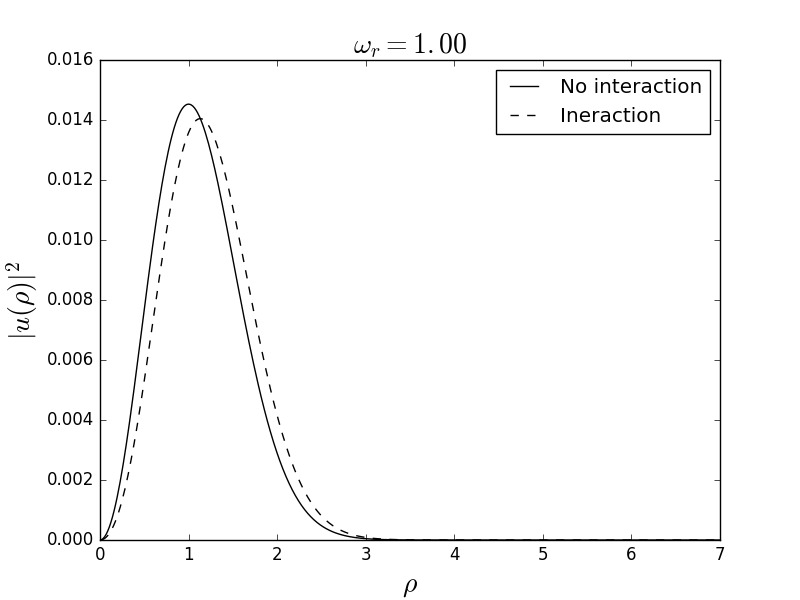
\includegraphics[width=0.45\textwidth]{../report/figures/freq100.png} 
		\caption{Comparison of the wavefunction with and without Coulomb interactions in a HO-potential where $\omega_r=1.00$}\label{fig:fq100}
	\end{figure}
	\begin{figure}[p]
		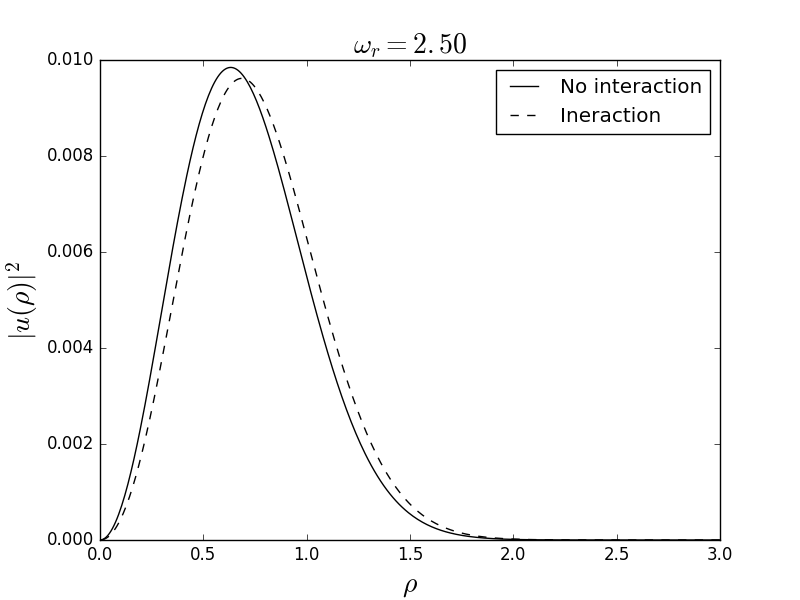
\includegraphics[width=0.45\textwidth]{../report/figures/freq250.png} 
		\caption{Comparison of the wavefunction with and without Coulomb interactions in a HO-potential where $\omega_r=2.50$}\label{fig:fq250}
	\end{figure}
	\begin{figure}[p]
		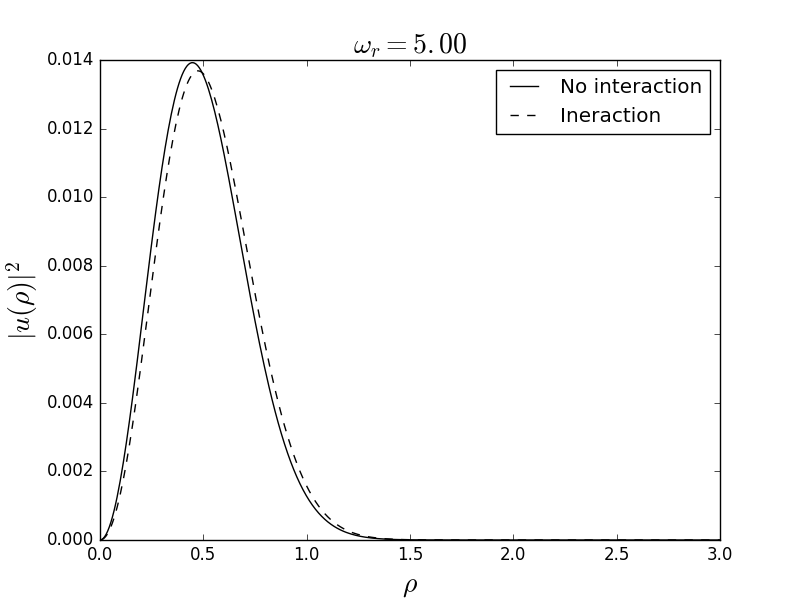
\includegraphics[width=0.45\textwidth]{../report/figures/freq500.png} 
		\caption{Comparison of the wavefunction with and without Coulomb interactions in a HO-potential where $\omega_r=5.00$}\label{fig:fq500}
	\end{figure}	%----------------------------------------------------------------------------
	\section{Summary and Conclusion}
	\label{sec:conclusion}
	A numerical experiment was done where \SE were solved iteratively by Jacobi's method. The algorithm was first compared to exact results of a simple system before calculated for more complex systems. The results of Table \ref{tbl:Coulomb} clearly show that the impact of the \CI on a system increases as the potential widens.\nl
	This may be used to design quantum dots that is able to contain more than one electron while still knowing roughly the energies of the electrons. Opening for more volume efficient manipulation of electons. 	%----------------------------------------------------------------------------
	%\twocolumn[]
	
\end{document}